\documentclass[12pt, letterpaper]{report}
\usepackage[a4paper, margin=0.7in, top=20mm, bottom=20mm]{geometry}
\usepackage{mathspec}
\usepackage[UTF8]{ctex}
\usepackage[colorlinks=true, linkcolor=black, urlcolor=blue]{hyperref}
\usepackage{listings}
\usepackage{xcolor}
\usepackage{graphicx}
\usepackage{xparse}
\usepackage{tcolorbox}
\usepackage{mdframed}

\graphicspath{ {./pics/} }

% ---- Code Section Style ----
\colorlet{mygray}{black!30}
\colorlet{mygreen}{green!60!blue}
\colorlet{mymauve}{red!60!blue}

\tcbuselibrary{breakable}
\NewDocumentCommand{\exercise}{ m +m }{
    {
        \edef\originalParIndent{\the\parindent}
        \begin{tcolorbox}[breakable,arc=0mm,boxrule=0.8pt]
            \setlength{\parindent}{\originalParIndent}
            \noindent
            \textbf{\large Exercise #1}
            \indent
            #2
        \end{tcolorbox}
    }
}

\lstdefinelanguage
   [x64]{Assembler}     % add a "x64" dialect of Assembler
   [x86masm]{Assembler} % based on the "x86masm" dialect
   % with these extra keywords:
   {morekeywords={CDQE,CQO,CMPSQ,CMPXCHG16B,JRCXZ,LODSQ,MOVSXD, %
                  POPFQ,PUSHFQ,SCASQ,STOSQ,IRETQ,RDTSCP,SWAPGS, %
                  rax,rdx,rcx,rbx,rsi,rdi,rsp,rbp, %
                  r8,r8d,r8w,r8b,r9,r9d,r9w,r9b, %
                  r10,r10d,r10w,r10b,r11,r11d,r11w,r11b, %
                  r12,r12d,r12w,r12b,r13,r13d,r13w,r13b, %
                  r14,r14d,r14w,r14b,r15,r15d,r15w,r15b}} % etc.


\lstset{
  backgroundcolor=\color{gray!10},  
  basicstyle=\ttfamily,
  columns=fullflexible,
  breakatwhitespace=false,      
  breaklines=true,                
  captionpos=b,                    
  commentstyle=\color{mygreen}, 
  extendedchars=true,              
  frame=single,                   
  keepspaces=true,             
  keywordstyle=\color{blue},                    
  numbers=none,                
  numbersep=5pt,                   
  numberstyle=\tiny\color{blue}, 
  rulecolor=\color{mygray},        
  showspaces=false,               
  showtabs=false,                 
  stepnumber=5,                  
  stringstyle=\color{mymauve},    
  tabsize=3,                      
  title=\lstname                
}

\lstdefinestyle{CStyle}{  
    % commentstyle=\color{mGreen},
    % keywordstyle=\color{magenta},
    % numberstyle=\tiny\color{mGray},
    % stringstyle=\color{mPurple},
    basicstyle=\footnotesize,
    breakatwhitespace=false,                              
    showstringspaces=false,
    language=C
}

\lstdefinestyle{AssemblyStyle}{  
    basicstyle=\footnotesize,
    breakatwhitespace=false,                              
    showstringspaces=false,
    language=[x64] Assembler
}


\lstdefinestyle{MakeFileStyle}{  
    basicstyle=\footnotesize,
    breakatwhitespace=false,                              
    showstringspaces=false,
    language=[gnu] make
}


% ----------------------------


\setcounter{chapter}{0}
\setlength{\parindent}{2em}
\setmainfont{Times New Roman}
\setcounter{tocdepth}{1}
\setcounter{secnumdepth}{1}

\title{MIT6.828 Lab2: Memory Management}
\author{Zhuofan Zhang}
\date{Jan 2022}



\begin{document}
\maketitle
% ---- Contents ----
\pagenumbering{roman}
\renewcommand\contentsname{\Huge Contents}
\tableofcontents{}
% ------------------


% ---- Part A ---------------------------------
\newpage
\pagenumbering{arabic}
\chapter[\Large Physical Page Management]{Physical Page Management}
本次 Lab 的内容主要分为两个部分,第一个部分是对可用物理内存的管理,第二个部分是虚拟内存的管理。\par
操作系统负责对可用物理内存的管理。JOS 的物理页使用 PageInfo 结构相关数据(数组/空闲链表)进行物理内存管理。
PageInfo 数组(pages)是对整个物理地址空间(32位,4GB)的映射:将整个物理地址空间按4KB-page划分,则每个单页
可由pages对应下标的 PageInfo 结构唯一指代(原理可见 pmap.h/page2pa 的实现)。\par 
\quad \par 
\exercise{1}{
        \par 
        \noindent {In the file kern/pmap.c, you must implement code 
        for the following functions:}
        \quad \par 
        \noindent \textbf{boot\_alloc() } \par
        \noindent \textbf{mem\_init() (only up to the call to check\_page\_free\_list(1))} \par
        \noindent \textbf{page\_init()} \par
        \noindent \textbf{page\_alloc()} \par
        \noindent \textbf{page\_free()} \par
        \quad \par 
        \noindent {check\_page\_free\_list() and check\_page\_alloc() test your physical page
        allocator. You should boot JOS and see whether check\_page\_alloc() reports success. 
        Fix your code so that it passes. You may find it helpful to add your own assert()s 
        to verify that your assumptions are correct.} \par
}
根据题目要求,我们依次实现上述函数。\par 
对于 \textbf{boot\_alloc} 函数,根据注释提示可知其为系统启动初期的 physical-page allocator,协助完成初始化工作。
函数中使用了一个变量 end,我们从内核的链接脚本(kernel.ld)中可以定位到它的位置,即.BSS段的末尾;根据注释提示,
end 表示第一处未被 kernel 使用的\underline{虚拟地址}。由 Lab1 可知内核被链接至高地址位(0xf0100000开始的4MB区域),
因此也许保证在这个阶段分配的物理内存不超过4MB,需要对分配是否越界进行检查。明确上述要求后,我们即可实现该函数:
\newpage

\lstset{style=CStyle}
\setmainfont{Consolas}
\begin{lstlisting}
static void *
boot_alloc(uint32_t n)
{
    static char *nextfree;	// virtual address of next byte of free memory
    char *result;

    // Initialize nextfree if this is the first time.
    // 'end' is a magic symbol automatically generated by the linker,
    // which points to the end of the kernel's bss segment:
    // the first virtual address that the linker did *not* assign
    // to any kernel code or global variables.
    if (!nextfree) {
        extern char end[];
        nextfree = ROUNDUP((char *) end, PGSIZE);
    }

    // Allocate a chunk large enough to hold 'n' bytes, then update
    // nextfree.  Make sure nextfree is kept aligned
    // to a multiple of PGSIZE.
    //
    // LAB 2: Your code here.
    result = nextfree;
    if(n > 0)
        nextfree = ROUNDUP(nextfree + n, PGSIZE);
    else if(n < 0)
        // n < 0: should not come here
        panic("boot_alloc: parameter n < 0.");
    
    // fix me: need to be explained
    if(PADDR(nextfree) >= 0x400000)
        panic("boot_alloc: run out of mem.");

    return result;
}
\end{lstlisting}
\setmainfont{Times New Roman}
\quad \par

\textbf{mem\_init} 函数是被内核 i386\_init() 调用的函数,用来完成内核内存管理的初始化;
本节仅需完成物理内存管理相关的部分。\par 
根据本节开头我们提到的物理内存管理方法,我们首先需要创建管理物理页的数组pages。由于pages本身也需要
占用内存,我们利用上一步实现的 boot\_alloc 分配内存并将pages进行0初始化。需要注意的是数组大小(npages)由 
i386\_detect\_memory 调用得到,它负责检查系统可用的物理内存大小。根据上述分析,我们实现 mem\_init 中初始化
pages部分的内容:\par 
\newpage
\lstset{style=CStyle}
\setmainfont{Consolas}
\begin{lstlisting}
void
mem_init(void)
{
    ...

    // Find out how much memory the machine has (npages & npages_basemem).
    i386_detect_memory();

    ...

    //////////////////////////////////////////////////////////////////////
    // Allocate an array of npages 'struct PageInfo's and store it in 'pages'.
    // The kernel uses this array to keep track of physical pages: for
    // each physical page, there is a corresponding struct PageInfo in this
    // array.  'npages' is the number of physical pages in memory.  Use memset
    // to initialize all fields of each struct PageInfo to 0.
    // Your code goes here:
    pages = (struct PageInfo *) boot_alloc(npages * sizeof(struct PageInfo));
    memset(pages, 0, npages * sizeof(struct PageInfo));

    ...
}
\end{lstlisting}
\setmainfont{Times New Roman}
\quad \par

上一步实现的代码中,我们可以看到在为pages分配内存并进行0初始化后,mem\_init 调用了真正
对pages及空闲列表page\_free\_list进行初始化的 
\textbf{page\_init} 。由于实际上系统运行至这一步时已经使用了一部分物理页,
因此我们必须根据系统当前的状态正确设置页内容,并将空闲页放入空闲列表。根据 page\_init 中的提示,我们完成代码如下。
其中比较需要关注的是 extended memory 空闲部分的初始化,第三步除了设置IO hole不空闲外,也需设置已经被使用的物理页,
而确定当前已用物理页位置末端(以虚拟地址表示)的方法是对 boot\_alloc 的零调用:\par 
(注:该部分内容可以结合 Lab1 中给出的 FIGURE: The PC's Physical Address Space 理解)\par 
\newpage
\lstset{style=CStyle}
\setmainfont{Consolas}
\begin{lstlisting}
void
page_init(void)
{
    // The example code here marks all physical pages as free.
    // However this is not truly the case.  What memory is free?
    //  1) Mark physical page 0 as in use.
    //     This way we preserve the real-mode IDT and BIOS structures
    //     in case we ever need them.  (Currently we don't, but...)
    //  2) The rest of base memory, [PGSIZE, npages_basemem * PGSIZE)
    //     is free.
    //  3) Then comes the IO hole [IOPHYSMEM, EXTPHYSMEM), which must
    //     never be allocated.
    //  4) Then extended memory [EXTPHYSMEM, ...).
    //     Some of it is in use, some is free. Where is the kernel
    //     in physical memory?  Which pages are already in use for
    //     page tables and other data structures?
    //
    // Change the code to reflect this.
    // NB: DO NOT actually touch the physical memory corresponding to
    // free pages!
    // 1) Mark physical page 0 as in use
    pages[0].pp_ref = 1;
    // 2) Base-memory
    size_t i;
    for (i = 1; i < npages_basemem; i++) {
        pages[i].pp_ref = 0;
        pages[i].pp_link = page_free_list;
        page_free_list = &pages[i];
    }
    // 3) IO hole + pages that have been used
    int hole_and_used = npages_basemem + 
                        ((EXTPHYSMEM - IOPHYSMEM) + 
                        PADDR(boot_alloc(0)))/PGSIZE;
    for(; i < hole_and_used; i++)
        pages[i].pp_ref = 1;

    // 4) extended memory
    for(; i < npages; i++)
    {
        pages[i].pp_ref = 0;
        pages[i].pp_link = page_free_list;
        page_free_list = &pages[i];
    }
}
\end{lstlisting}
\setmainfont{Times New Roman}
\quad \par

实现了pages及page\_free\_list的初始化后,就可以进一步实现分配和回收页的函数:
\textbf{page\_alloc} 与 \textbf{page\_free} 。注意到实现物理页分配时,对页面进行初始化时
\underline{需要获得物理页的虚拟地址}(C语言中地址均匀虚拟地址),
根据提示使用 page2kva 实现。page2kva 本身的实现是使用 page2pa 得到物理页的实际地址,再根据当前
的映射使用 KADDR 转化为虚拟地址。
\lstset{style=CStyle}
\setmainfont{Consolas}
\begin{lstlisting}
struct PageInfo *
page_alloc(int alloc_flags)
{
    // Fill this function in
    if(!page_free_list)
        return NULL;

    struct PageInfo *alloc_page = page_free_list;
    page_free_list = page_free_list->pp_link;
    alloc_page->pp_link = NULL;

    if(alloc_flags & ALLOC_ZERO)
        memset(page2kva(alloc_page), 0, PGSIZE);

    return alloc_page;
}

void
page_free(struct PageInfo *pp)
{
	// Fill this function in
	// Hint: You may want to panic if pp->pp_ref is nonzero or
	// pp->pp_link is not NULL.
	if(pp->pp_ref != 0 || pp->pp_link != NULL)
		panic("page_free: pp_ref != 0");
	
	pp->pp_link = page_free_list;
	page_free_list = pp;

}
\end{lstlisting}
\setmainfont{Times New Roman}

% ------------------------------------------------------------

\chapter[\Large Virtual Memory]{Virtual Memory}

\exercise{2}{
        \par 
        \noindent{
            Look at chapters 5 and 6 of the Intel 80386 Reference Manual, 
            if you haven't done so already. Read the sections about page translation 
            and page-based protection closely (5.2 and 6.4). 
            We recommend that you also skim the sections about segmentation; 
            while JOS uses the paging hardware for virtual memory and protection, 
            segment translation and segment-based protection cannot be disabled on the x86, 
            so you will need a basic understanding of it.} \par 
}
\quad \par 
这一节内容需要我们构建虚拟内存管理的基本设施,Exercise2为我们提供了80386处理器内存管理模式的相关材料。
阅读相关材料后,我们可以整理出处理器为我们提供的内存管理机制:分段/分页。

\section[\large Virtual, Linear, and Physical Addresses]{Virtual, Linear, and Physical Addresses}
在x86体系中,我们可以定义3种地址:虚拟地址(Virtual Address, VA)[也称Logical Address],
线性地址(Linear Address, LA)与物理地址(Physical Address, PA)。\par
对于用户而言,可见的只有VA,而数据在物理内存中的实际地址是PA。x86的典型地址翻译流程如下图所示,
其中VA $\rightarrow$ LA 的过程为 \textsl{分段(Segmentation)} 机制,LA $\rightarrow$ PA 过程为 \textsl{分页(Paging)} 机制。\par
关于分页与分段的详细内容不在此处展开,但需知道:JOS 并不使用分段机制,但x86系统并没有显式关闭分段的方法。因此,
在设置 Segment Descript Table 时,JOS 将段基址设置为0,并将 LIMIT 设置为 0xffffffff,即将整个物理地址空间视为
一段,在这种情况下VA = LA。设置的过程在 Lab1 中的 boot 阶段完成(boot.S)。\par 
{
\centering
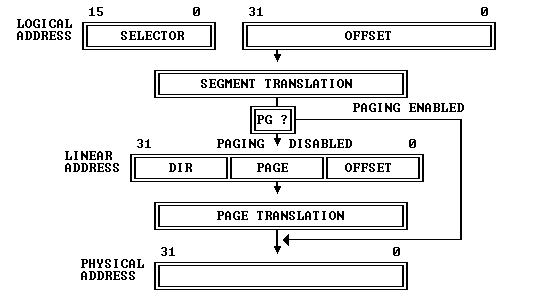
\includegraphics[width=0.8\textwidth]{AddressTranslationOverview}
}
\quad \par 
\quad \par 
\exercise{3}{
        \par 
        \quad {
            While GDB can only access QEMU's memory by virtual address, 
            it's often useful to be able to inspect physical memory 
            while setting up virtual memory. 
            Review the QEMU monitor commands from the lab tools guide, 
            especially the xp command, which lets you inspect physical memory. 
            \underline{To access the QEMU monitor, press Ctrl-a c in the terminal} 
            (the same binding returns to the serial console).
        } \par

        \quad {
            Use the \textbf{xp} command in the QEMU monitor and the x command in GDB 
            to inspect memory at corresponding physical and virtual addresses 
            and make sure you see the same data.
        } \par

        \quad {
            Our patched version of QEMU provides an \textbf{info pg} command that may also prove useful: 
            it shows a compact but detailed representation of the current page tables, 
            including all mapped memory ranges, permissions, and flags. 
            Stock QEMU also provides an \textbf{info mem} command that shows an overview 
            of which ranges of virtual addresses are mapped and with what permissions.
        } \par 
}
\quad \par
这一个练习的第一个要求与 Lab1 类似,要求我们观察虚拟地址与其实际映射到的物理地址的内容是否一致
(即虚拟内存映射是否成功)。与 Lab1 不同,此处采用更泛用的方法:使用GDB观察PA,使用QEMU-monitor观察
VA。根据提示,我们在gdb设置内存映射成功后的位置检查,可以看到VA及其对应的PA内容的一致性:\par 

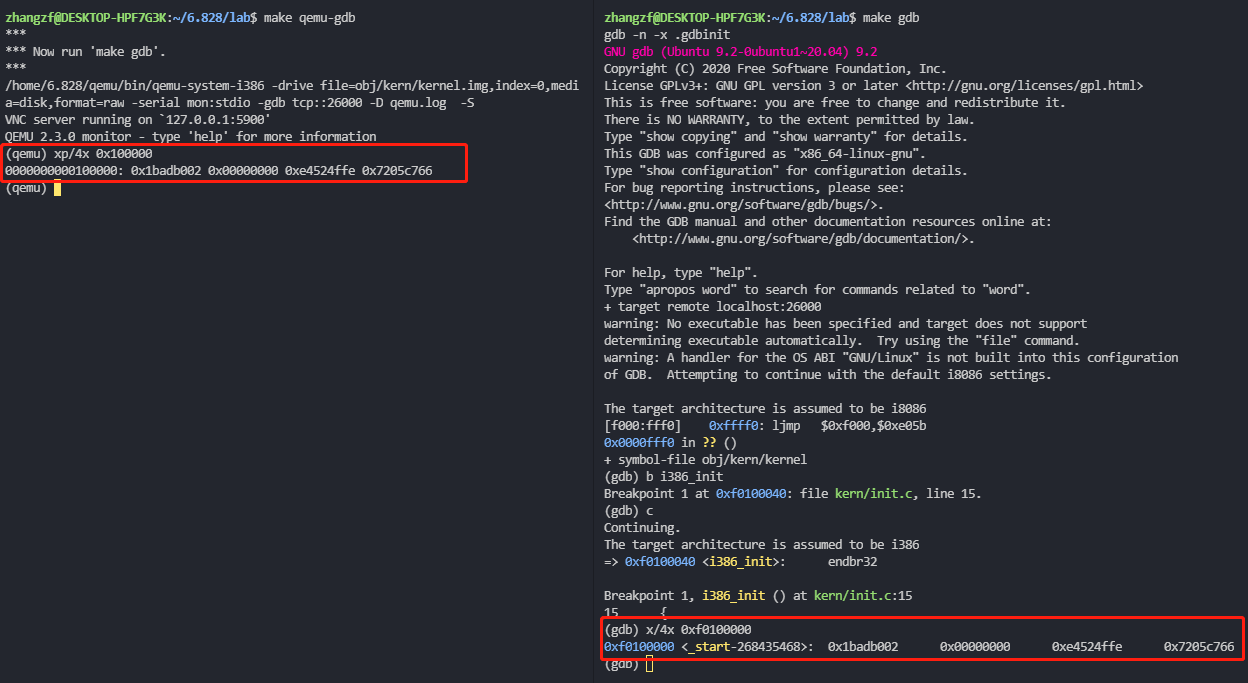
\includegraphics[width=0.85\textwidth]{pa_va}

\quad \par 
此外,我们还根据提示,使用 \textbf{info pg/mem} 命令查看页表情况与内存权限情况:\par 
\quad \par 

\lstset{style=AssemblyStyle}
\setmainfont{Consolas}
\begin{lstlisting}
(qemu) info pg
VPN range     Entry         Flags        Physical page
[00000-003ff]  PDE[000]     ----A----P
    [00000-000ff]  PTE[000-0ff] --------WP 00000-000ff
    [00100-00100]  PTE[100]     ----A---WP 00100
    [00101-00111]  PTE[101-111] --------WP 00101-00111
    [00112-00112]  PTE[112]     ---DA---WP 00112
    [00113-003ff]  PTE[113-3ff] --------WP 00113-003ff
[f0000-f03ff]  PDE[3c0]     ----A---WP
    [f0000-f00ff]  PTE[000-0ff] --------WP 00000-000ff
    [f0100-f0100]  PTE[100]     ----A---WP 00100
    [f0101-f0111]  PTE[101-111] --------WP 00101-00111
    [f0112-f0112]  PTE[112]     ---DA---WP 00112
    [f0113-f03ff]  PTE[113-3ff] --------WP 00113-003ff
(qemu) info mem
0000000000000000-0000000000400000 0000000000400000 -r-
00000000f0000000-00000000f0400000 0000000000400000 -rw
\end{lstlisting}
\setmainfont{Times New Roman}
\quad \par

本节的最后,Lab 还简要介绍了 JOS 中地址类型的 typedef。JOS 将地址类型区分为
虚拟地址(uintptr\_t)与物理地址(physaddr\_t),它们均为 uint32\_t 的typedef。
由于C中所有出现的“地址”均为虚拟地址,故其中uintptr\_t可以被解引用使用,而physaddr\_t
不应被解引用,它仅作为物理地址字面值被使用,对其解引用将引发UB。\par 


\end{document}